\chapter{\ifenglish Introduction\else บทนำ\fi}

\section{\ifenglish Project rationale\else ที่มาของโครงงาน\fi}
ในแต่ละปีการศึกษา สำนักทะเบียนและประมวลผล มหาวิทยาลัยเชียงใหม่ จำเป็นจะต้องจัดทำร่างปฏิทินการศึกษาสำหรับปีการศึกษาถัดไป เพื่อให้กรรมการบริหารมหาวิทยาลัยอนุมัติล่วงหน้า

ปฏิทินการศึกษาประกอบไปด้วยกำหนดการของกิจกรรมการศึกษาต่างๆ เช่น วันเปิดภาคเรียน วันลงทะเบียนเรียน วันสุดท้ายของการถอนกระบวนวิชา และวันสอบ เป็นต้น
%
กิจกรรมการศึกษาต่างๆ ส่วนใหญ่นั้นจะถูกกำหนดเป็นเงื่อนไขที่อ้างอิงกับวันเปิดภาคเรียน เช่น วันสุดท้ายของการเรียนการสอน จะถัดจากวันเปิดภาคเรียนประมาณ 16 สัปดาห์ จากนั้น จะเป็นการสอบปลายภาค ระยะเวลา 2 สัปดาห์ แล้วตามด้วยวันประกาศผลการศึกษา หลังจากสอบปลายภาควันสุดท้ายไปประมาณ 2 สัปดาห์
%
จะเห็นว่า หากกำหนดวันเปิดภาคการศึกษาให้ชัดเจนแล้ว กิจกรรมอื่นๆ จะสามารถจัดวางได้โดยอัตโนมัติ จึงทำให้การร่างปฏิทินการศึกษานั้นไม่ควรใช้เวลามากนัก

แต่ในความเป็นจริงแล้ว สำนักทะเบียนและประมวลผลยังขาดเครื่องมือที่จะอำนวยความสะดวกในการร่างปฏิทินการศึกษา ทำให้ต้องใช้เวลาในการสร้างแต่ละร่างถึง 2 สัปดาห์เป็นอย่างต่ำ
%
สาเหตุหลักๆ ในความล่าช้าดังกล่าว คือเงื่อนไขสำหรับกิจกรรมการศึกษาต่างๆ ที่ไม่ได้ระบุไว้เป็นลายลักษณ์อักษรให้ชัดเจน เพื่อที่จะสามารถนำมาใช้ซ้ำได้ ทำให้ผู้จัดทำร่างปฏิทินต้องกำหนดเงื่อนไขดังกล่าวในทุกๆ ปี ก่อนจะวางโครงร่างปฏิทินโดยการนับวันด้วยมือ
%
นอกจากนี้ หากกรรมการบริหารมหาวิทยาลัยมีมติให้แก้ไขร่างดังกล่าว ซึ่งอาจจะเกิดขึ้นได้หลายครั้งในแต่ละปีการศึกษา จะทำให้ผู้จัดทำร่างปฏิทินเสียเวลาเพิ่มเติมมากกว่าที่ควรจะเป็น เนื่องจากจะต้องเริ่มกระบวนการร่างปฏิทินใหม่ทั้งหมด
%
รวมไปปัญหาการที่จะแก้ไขวันหรือกิจกรรมในปฏิทินอย่างกระทัน ก็ยังไม่มีเครื่องมือที่จะช่วยแก้ปัญหาได้ หากกรรมการบริหารมหาวิทยาลัยเชียงใหม่ต้องการที่จะเปรียบเทียบหรือดูตัวอย่างของปฏิทินปีก่อนๆ แล้วนำมาแก้ไขเพียงบางส่วน ผู้จัดทำร่างปฏิทินก็จะต้องเตรียมเอกสารปฏิทินมาหลายฉบับ ซึ่งทำให้เกิดปัญหาให้แก่ผู้จัดทำร่างปฏิทินเป็นอย่างมาก

จากปัญหาการสร้างปฏิทินการศึกษาข้างต้น ผู้จัดทำโครงงานจึงมีแนวคิดที่จะสร้างโปรแกรมวางแผนปฏิทินการศึกษา มหาวิทยาลัยเชียงใหม่
%
เพื่อที่จะเป็นเครื่องมือที่จะช่วยให้ผู้จัดทำร่างปฏิทินของสำนักทะเบียนสามารถลดเวลาในการจัดทำปฏิทินลงได้
%
อีกทั้งยังสามารถเพิ่มความสะดวกในการจัดทำร่างปฏิทิน ไม่ว่าจะเป็นการเปลี่ยนแปลงวันกิจกรรมได้อย่างรวดเร็ว การแก้ไขร่างปฏิทินอย่างกระทันหัน การสร้างร่างปฏิทินหลายฉบับที่มีความคล้ายคลึงกัน โปรแกรมดังกล่าวก็สามารถตอบสนองได้

\paragraph{คำจำกัดความ}
\begin{enumerate}
    \item ผู้ใช้ (User) คือผู้ที่จะเป็นคนใช้ระบบนี้ ซึ่งในที่นี้จะหมายถึงบุคลากรของสำนักทะเบียนมหาวิทยาลัยเชียงใหม่ ที่รับผิดชอบในการจัดทำปฏิทินการศึกษาโดยเฉพาะ
    \item ปฏิทินการศึกษา หรือ ร่างปฏิทิน (Calendar) คือแบบร่างของปฏิทินการศึกษาในปีการศึกษานั้นๆ ที่ผู้ใช้เป็นคนจัดทำขึ้น โดยในผู้ใช้แต่ละคนจะสามารถสร้างร่างปฏิทินการศึกษาได้หลายร่างปฏิทิน
    \item วันเรียน (Study day) เป็นวันที่มีการเรียนการสอนของปฏิทินการศึกษา ในที่นี้จะเริ่มจากวันเปิดภาคการศึกษา ไปจนถึงปิดภาคการศึกษา
    \item วันหยุด (Holiday) เป็นวันที่ไม่มีการเรียนการสอน ซึ่งในที่นี้จะหมายถึงวันหยุดทุกรูปแบบ รวมถึงวันหยุดพิเศษ
    \item กำหนดการสำคัญ (Event) เป็นกำหนดการอื่นๆ นอกเหนือจากวันหยุด
    \item วันสอบ (Exam) เป็นวันที่มีการสอบ โดยหากปรากฏขึ้นในปฏิทินการศึกษา จะไม่นับว่าเป็นทั้งวันที่มีการเรียนการสอน และวันหยุด
    \item วันปิดเทอม เป็นวันหยุดโดยเริ่มจากวันปิดภาคเรียนของภาคก่อนหน้า ไปจนถึงวันเปิดภาคเรียนถัดไป
\end{enumerate}

เราได้ทราบมาว่าในแต่ละปฏิทินการศึกษาของแต่ละปีการศึกษานั้นมีความยุ่งยากและซับซ้อน แถมยังใช้เวลานานเป็นหลักสัปดาห์ เราจึงไปทำการพูดคุยกับบุคลากรของสำนักทะเบียนมหาวิทยาลัยเชียงใหม่เพื่อทราบถึงปัญหา โดยเราจะสรุปวิธีการสร้างร่างปฏิทินการศึกษาไปจนถึงการประกาศปฏิทินการศึกษาได้ดังนี้

\begin{figure}[h]
    \centering
    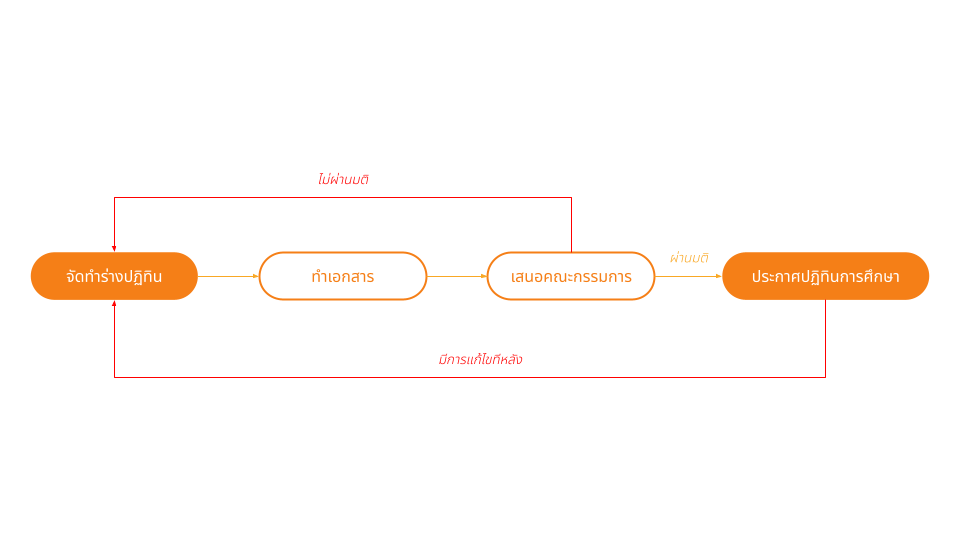
\includegraphics[width=1\textwidth]{create-draft.png}
    \caption{ขั้นตอนการทำร่างปฏิทินการศึกษา}
    \label{fig:user-flow-create-draft}
\end{figure}
จากภาพจะเห็นขั้นตอนการสร้างปฏิทินการศึกษานั้น ๆ และในแต่ละขั้นตอนจะมีความซับซ้อนในตัวของขั้นตอนนั้น ๆ อยู่ เราจึงทำการสรุปความซับซ้อนทั้งหมดของการสร้างร่างปฏิทินการศึกษาตามขั้นตอนดังนี้

\paragraph{1. การจัดทำร่างปฏิทิน}

\par การจัดทำร่างปฏิทินการศึกษาของมหาวิทยาลัยเชียงใหม่นั้นมีความซับซ้อนเนื่องจากในแต่ละวันของปฏิทินการศึกษาจะมีเงื่อนไขอยู่ ผู้จัดทำจะต้องเริ่มจากการกำหนดวันเปิดภาคการศึกษาที่ 1 เพื่อเป็นวันอ้างอิงในการวางวันที่มีกำหนดการอื่นๆ หรือกำหนดการในปฏิทินการศึกษาอื่นๆ และในการวางกำหนดการในปฏิทินการศึกษาอื่นๆ ก็มีการอ้างอิงกับกำหนดการอื่นๆอีกเช่นเดียวกันตัวอย่างเช่น วันสุดท้ายของการส่งผลการศึกษาจะเกิดขึ้นหลังจากวันสอบปลายภาควันสุดท้าย 9 วัน และวันสอบวันสุดท้ายจำเป็นจะต้องห่างจากวันเปิดภาคเรียน 17 สัปดาห์ และยังมีกำหนดการอื่นๆที่มีเงื่อนไขอ้างอิงกับวันที่มีกำหนดการอื่นๆอีก โดยรวมแล้วมีมากกว่า 70 กำหนดการในแต่ละปี และอาจมีเพิ่มลดได้อีกขึ้นอยู่กับสถาณการณ์และการวางแผนในปีการศึกษานั้น


\par ผู้จัดทำยังต้องวางวันหยุดที่มีการหยุดเป็นประจำทุกปีของราจกิจจานุเบกษา รวมถึงวันหยุดที่เป็นวันหยุดจันทรคติด้วย ซึ่งในวันหยุดจันทรคตินั้นไม่มีประกาศที่แน่นอนในแต่ละปี และยังไม่มีประกาศในที่ที่เป็นทางการของวันหยุดจันทรคตินั้นๆด้วย ซึ่งอาจเกิดการเปลี่ยนแปลงได้ในภายหลัง


\par หลังจากที่ผู้จัดทำการวางกำหนดการทุกอย่างสำเร็จแล้ว ผู้จัดทำต้องทำการนับวันเรียนเป็นรายเทอมเพื่อนำมาคำนวนชั่วโมงแบบสรุปทั้งภาคเรียนตั้งแต่วันจันทร์ถึงวันศุกร์ โดยการนับคาบเรียนเพื่อคำนวนชั่วโมงนั้นจะเริ่มนับจากวันเปิดภาคเรียนของภาคเรียนนั้นๆไปจนถึงวันปิดภาคเรียนของภาคเรียนนั้นๆ โดยนับทั้งวันเป็นหนึ่งคาบเรียนต่อ1วิชา เนื่องจากในแต่ละวิชามีคาบเรียนวิชานั้นๆได้แค่ 1 คาบ และนำมาทำการคูณกับชั่วโมงต่อคาบเรียนในวันนั้น เช่น หากวันจันทร์มีวันเรียน 15 คาบ และใน 1 คาบ มีเวลา 1 ชั่วโมง 30 นาที ในภาคการศึกษานี้จะมีชั่วโมงเรียนวันจันทร์อยู่ 22 ชั่วโมง 30 นาที


\par โดยการนับเงื่อนไขที่กล่าวมาข้างต้น ผู้จัดทำจะเริ่มจากการเขียนกำหนดการในกระดาษ และนับเงื่อนไขของกำหนดการที่มีวันอ้างอิงโดยอ้างอิงจากปฏิทินการศึกษาปีก่อนๆทีละกำหนดการ จนหมดภาคเรียน และอาจมีปรับเปลี่ยนตามความเหมาะสมและตามประกาศต่างๆของรัฐบาล และยังต้องมีการเปลี่ยนแปลงหลังจากประกาศมีการเปลี่ยนแปลงด้วย

\paragraph{2. การทำเอกสาร}\enskip

\par หลังจากการทำร่างปฏิทินแล้ว ผู้จัดทำต้องจัดทำเอกสารสรุปออกมาเป็น 6 เอกสารหลักๆ ที่เกี่ยวกับปฏิทินการศึกษาร่างนั้น ได้แก่

\begin{figure}[h]
    \centering
    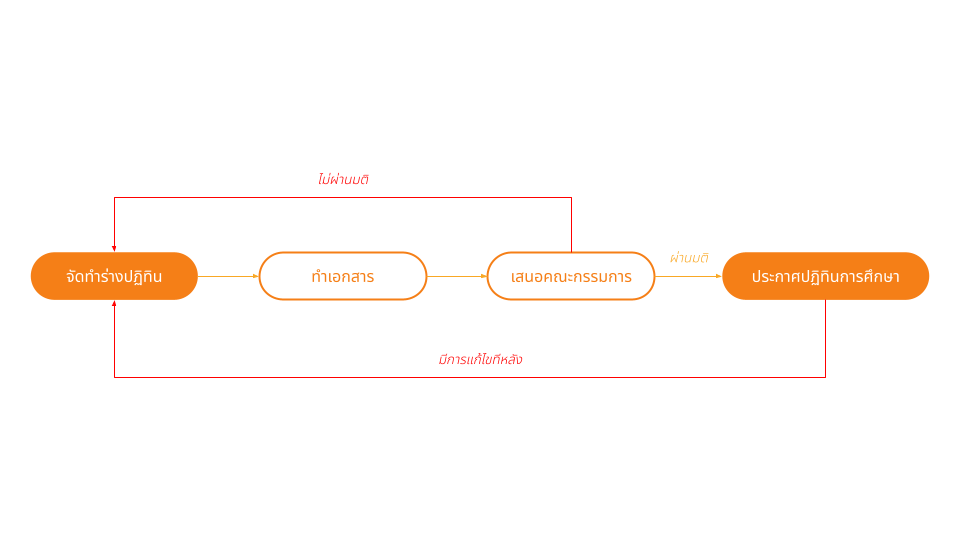
\includegraphics[width=1\textwidth]{create-draft.png}
    \caption{เอกสารที่ 1}
    \label{fig:academic-draft}
\end{figure}

\par เอกสาร	1 โครงร่างปฏิทินการศึกษา ในเอกสารโครงร่างปฏิทินการศึกษานั้นจะเป็นตารางของการสรุประยะเวลาของกิจกรรมใน 1 ภาคการศึกษา
โดยกำหนดการที่จะนำไปทำการใส่ลงในตารางได้แก่ วันรายงานตัว วัน pre-college วันลงทะเบียนเรียนภาคการศึกษาที่ 1 เวลาเรียนทั้งหมด วันสอบกลางภาค วันสอบปลายภาค วันตรวจข้อสอบ วันส่งผลการศึกษา วันประมวลผล วันประกาศผล \enskip

\begin{figure}[h]
    \centering
    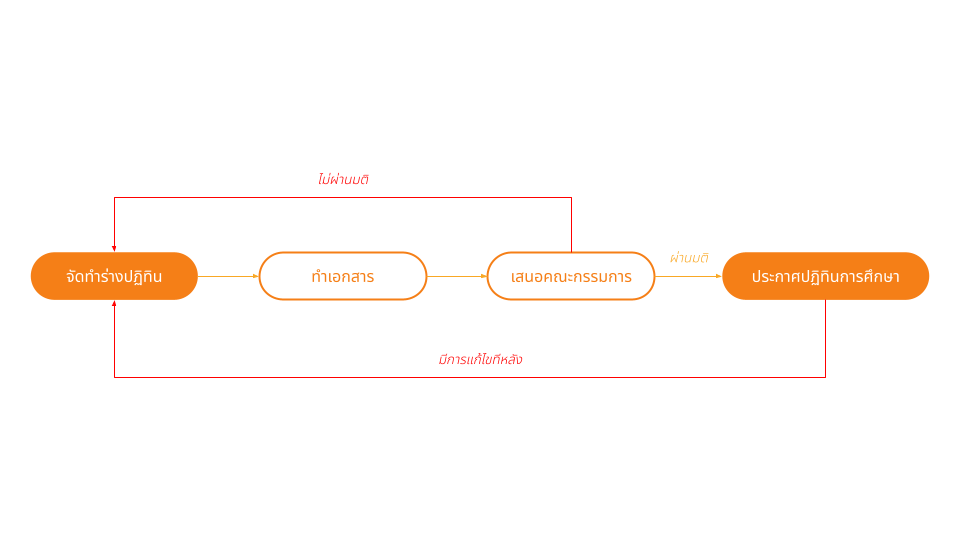
\includegraphics[width=1\textwidth]{create-draft.png}
    \caption{เอกสารที่ 2}
    \label{fig:duration-calendar}
\end{figure}
\par เอกสาร 2 ระยะเวลาของปฏิทินการศึกษา
ในที่นี้จะรวมสรุประยะเวลาของปฏิทินการศึกษาไว้ โดยมีกำหนดการสำคัญของปฏิทินการศึกษาบางกำหนดการอยู่ในเอกสารนี้ ได้แก่ วันรายงานตัวนักศึกษาใหม่ วันลงทะเบียนเรียน และสรุปเวลาเรียนรวมถึงวันสอบปลายภาคและวันสอบไล่ในแต่ละภาคการศึกษา \enskip

\begin{figure}[h]
    \centering
    
\includegraphics[width=1\textwidth]{pic3.1.jpg}
    \caption{เอกสารที่ 3}
    \label{fig: conclude-per-semester}
\end{figure}
\par เอกสาร 3 ระยะเวลาในการปฏิบัติงานระหว่างภาคการศึกษา
จะสรุปกำหนดการสำคัญในระหว่างภาคการศึกษา โดยเริ่มจากวันสอบไล่ของภาคการศึกษานั้นๆ ไปจนถึงวันที่สภาวิชาการให้ความเห็นชอบในการสำเร็จการศึกษา


\begin{figure}[h]
    \centering
    
\includegraphics[width=1\textwidth]{pic3.1.jpg}
    \caption{เอกสารที่ 4}
    \label{fig: conclude-study-week}
\end{figure}
\par เอกสารที่ 4 สรุประยะเวลาที่ใช้สำหรับการเรียนการสอน
ในเอกสารนี้ต้องทำการสรุประยะเวลาที่ใช้สำหรับการเรียนการสอนในแต่ละภาคการศึกษา รวมถึงสรุปชั่วโมงเรียนของทั้งภาคเรียนเป็นรายวัน รวมถึงสัปดาห์เรียน และคาบเรียนแต่ละคาบในแต่ละวันตั้งแต่จันทร์ถึงศุกร์ มีการสรุปวันหยุดราชการที่กำหนดอยู่ในช่วงระยะเวลาของภาคการศึกษานั้นๆเป็นรายวัน และยังต้องบอกวันเริ่มต้นไปจนถึงวันสิ้นสุดของภาคการศึกษานั้น

\begin{figure}[h]
    \centering
    
\includegraphics[width=1\textwidth]{pic3.1.jpg}
    \caption{เอกสารที่ 5}
    \label{fig: academic-calendar-draft}
\end{figure}
\par เอกสารที่ 5 ร่างปฏิทินการศึกษา
ในเอกสารนี้จะเป็นร่างประกาศปฏิทินการศึกษาสำหรับนักศึกษาทั่วไปแยกเป็นรายภาคการศึกษา โดยจะสรุปกำหนดการสำคัญและวันสอบในแต่ละภาคการศึกษานั้น รวมถึงบอกวันเวลาของกำหนดการสำคัญที่นำมาสรุป

\begin{figure}[h]
    \centering
    
\includegraphics[width=1\textwidth]{pic3.1.jpg}
    \caption{เอกสารที่ 6}
    \label{fig: holiday-draft}
\end{figure}
\par เอกสารที่ 6 สรุปวันหยุดและวันหยุดชดเชย
ในเอกสารนี้จะเป็นเอกสารที่สรุปวันหยุดและวันหยุดชดเชยทั้งหมดในปีการศึกษานั้นโดยนับจากวันเปิดภาคเรียนแรกของปีการศึกษานั้นไปจนถึงปิดภาคเรียนสุดท้ายในทุกภาคการศึกษา โดยไม่นับวันปิดเทอม


%     ในปัจจุบันปฏิทินการศึกษาของมหาวิทยาลัยเชียงใหม่นั้นจัดทำโดยทางสำนักทะเบียนของมหาวิทยาลัยเชียงใหม่ 
% โดยที่ในการที่จะสร้างปฏิทินขึ้นมาได้นั้น จะต้องมีการร่างโครงร่างของปฏิทินออกมา โดยที่ในการที่จะร่างปฏิทินนั้ก็จะต้องมีเงื่อนไขในการส้รางปฏิทินต่างๆ ไม่ว่าจะเป็น การกำหนดวันเปิดภาคเรียน การกำหนดระยะเวลาของคาบเรียน วันปิดภาคเรียน ไปจนถึงวันลงทะเบียน 
% เราได้พบปัญหาว่าใน 1 ปฏิทินการศึกษานั้น ใช้เวลาในการร่างปฏิทินไม่ต่ำกว่า 2 สัปดาห์ เนื่องจากทางผู้จัดทำต้องกำหนดเงื่อนไขที่ได้กล่าวข้างต้น ถึงจะทำการวางโครงร่างของปฏิทินได้
% และเมื่อสามารถวางโครงร่างได้แล้วก็จะต้องนำโครงร่างไปส่งให้เป็นที่พิจารณาแก่คณะกรรมการบริหารของมหาวิทยาลัยเชียงใหม่ ซึ่งจะทำให้ต้องมีการแก้ไขอยู่หลายๆครั้ง จึงทำให้การทำปฏิทินวันเปิดภาคเรียนนั้นใช้เวลานานมากเกินไป เราจึงได้เล็งปัญหาของการสร้างปฏทินการศึกษา
% ซึ่งจัดทำโดยสำนักทะเบียนมหาวิทยาลัยเชียงใหม่ จึงได้เกิดเป็นโปรแกรมวางแผนปฏิทินการศึกษา มหาวิทยาลัยเชียงใหม่



\section{\ifenglish Objectives\else วัตถุประสงค์ของโครงงาน\fi}
Chiang Mai University's academic calendar planner (CMU ACAD)  ถูกพัฒนาขึ้นเพื่อ
\begin{enumerate}
    \item เพื่อลดระยะเวลาในการสร้างร่างปฏิทินการศึกษาของสำนักทะเบียนและวัดผล มหาวิทยาลัยเชียงใหม่
    \item เพื่อสรุปรายละเอียดในการสร้างร่างปฏิทินการศึกษาในร่างปฏิทินการศึกษานั้นๆที่ถูกสร้างขึ้นมาเพื่อทำให้นำไปสรุปเอกสารได้ง่ายขึ้น
    \item สร้างระบบที่สามารถระบุเงื่อนไขต่าง ๆ ที่จําเป็นต่อการสร้าง ปฏิทินการศึกษา และสามารถแก้ไขได้ตามความต้องการ
    \item เพื่อสร้างระบบที่สามารถคัดลอกและทำซ้ำของปฏิทินได้ เมื่อต้องการที่จะแก้ปฏิทินหลายๆ ฉบับ และต้องเปลี่ยนการเปลี่ยนแปลงเพียงบางส่วน
\end{enumerate}

\section{\ifenglish Project scope\else ขอบเขตของโครงงาน\fi}
Chiang Mai University's academic calendar planner จะเป็น web application ทำงานบน web browser เท่านั้น เพื่อให้สามารถเข้าสู่ระบบจากคอมพิวเตอร์เครื่องใดก็ได้ และผู้ที่เข้าถึงได้และจำกัดสิทธิ์เข้าถึงได้คือบุคลากรของสำนักทะเบียนและวัดผล มหาวิทยาลัยเชียงใหม่
\subsection{\ifenglish Hardware scope\else ขอบเขตด้านฮาร์ดแวร์\fi}
\begin{enumerate}
    \item CMU ACAD ออกแบบมาเพื่อทำงานในคอมพิวเตอร์ (PC) เท่านั้น เนื่องจากเป็น web application ที่จำเป็นต้องใช้ขนาดจอที่ใหญ่ในการแก้ไขร่างปฏิทิน
\end{enumerate}

\subsection{\ifenglish Software scope\else ขอบเขตด้านซอฟต์แวร์\fi}
\begin{enumerate}
    \item การ export จะไม่ออกมาเป็นเอกสารที่เป็นทางการ  แต่จะมาในรูปแบบสรุปกำหนดการสำคัญและวันหยุดในร่างปฏิทินนั้นในรูปแบบ xlsx เพื่อนำไปใช้ทำเอกสารที่เป็นทางการ
    \item โปรแกรมวางแผนนี้จะเพิ่มวันหยุดและกำหนดการให้โดยอัตโนมัติเมื่อสร้างร่างปฏิทินในปีการศึกษานั้นขึ้นมา แต่กิจกรรมที่นักศึกษา เป็นฝ่ายจัดจะไม่นับลงไปด้วย เช่น กิจกรรม Sports Day กิจกรรม Freshy Night เป็นต้น
    \item เมื่อเริ่มสร้างปฏิทินแล้วโปรแกรมจะทำการวางวันหยุดและกำหนดการให้แบบอัติโนมัติ โดยวันหยุดที่ทำการวางให้นี้เป็นวันหยุดที่เป็นไปตามราชกิจจานุเบกษาและวันหยุดที่ทางมหาลัยมีขึ้นเป็นประจำทุกปีเท่านั้น ยกเว้นวันหยุดที่มีความไม่แน่นอนหรือวันหยุดจันทรคติ
    \item ไม่มี responsive สำหรับมือถือ เนื่องจากการออกแบบแอพพลิเคชั่นนี้มีไว้สำหรับทำปฏิทินเอกสารบนหน้าคอมพิวตอร์เท่านั้น และในการแก้ไขร่างปฏิทินของปฏิทินการศึกษานั้นที่ออกแบบมาให้ใช้กับหน้าจอใหญ่ (ไม่ต่ำกว่า 1440 x 1024 px)
    \item ผู้ใช้จะสามารถเข้าสู่ระบบได้จาก CMU Oauth ซึ่งเป็นระบบสำหรับให้บริการการยืนยันตัวตนจากส่วนกลาง
    \item ในเบื้องต้น ผู้พัฒนาได้ออกแบบหน้าการแก้ไขของเงื่อนไขปฏิทิน เพื่อเป็นฟังก์ชั่นที่จะนำเงื่อนไขไปใช้ในอนาคต
\end{enumerate}

\section{\ifenglish Expected outcomes\else ประโยชน์ที่ได้รับ\fi}
\begin{enumerate}
    \item สำนักทะเบียนและมหาวิทยาลัยสามารถลดเวลาในการทำร่างปฏิทินการศึกษาให้ใช้เวลาในการทําลดลง ซึ่งหากมีการแก้ไขเพิ่มเติมของคณะกรรมการของมหาวิทยาลัยจะทำให้แก้ไขร่างปฏิทินได้สะดวกขึ้นกว่าการร่างปฏิทินด้วยมือและทดในกระดาษ
    \item ลดเวลาในการทำเอกสารทางการต่างๆของสำนักทะเบียนเพื่อนำไปเสนอคณะกรรมการของมหาวิทยาลัย
    \item โปรแกรมวางแผนปฏิทินการศึกษานี้สามารถใช้ได้จริง และเป็นประโยชน์ในการออกปฏิทินของสำนักทะเบียนและประมวลผล มหาวิทยาลัยเชียงใหม่
\end{enumerate}

\section{\ifenglish Technology and tools\else เทคโนโลยีและเครื่องมือที่ใช้\fi}

\subsection{\ifenglish Hardware technology\else เทคโนโลยีด้าน hardware\fi}
\begin{enumerate}
    \item Desktop computer
    \item Macbook Air 2021
    \item Asus tuf gaming fx505dt
\end{enumerate}
\CIreply{wording style between items not parallel}

\subsection{\ifenglish Software technology\else เทคโนโลยีด้านซอฟต์แวร์\fi}
\begin{enumerate}
    \item ใช้ Figma\cite{Figma} เป็นเครื่องมือที่นำไปใช้ในการออกแบบหน้าแสดงผล(user interface) รวมถึงการทดสอบหน้าแสดงผล และ ประสบการณ์การใช้งานของผู้ใช้ (user experience) ก่อนที่จะเริ่มเขียนแบบโค๊ด
    \item HTML\cite{HTML} ย่อมาจาก HyperText Markup Language เป็น ภาษาคอมพิวเตอร์ท่ี ใช้สร้างหน้าเว็บในรูป แบบของไฟล์ HTML (คือไฟล์ที่มีนามสกุลเป็น .htm หรือ .html) ซึ่งมีเว็บเบราว์เซอร์เป็นโปรแกรมที่ใช้ แปลงไฟล์HTML เพื่อ แสดงผลในรูปของหน้าเว็บ ไฟล์HTML บันทึกในรูปของไฟล์เอกสาร (text file) ที่สามารถถูกสร้างจากโปรแกรมสร้างไฟล์ ข้อความ เช่น Notepad หรือ word processing ทั่วๆ ไป ซึ่งลักษณะของไฟล์HTML ประกอบไปด้วยแท็กต่างๆ ที่เป็นคําสั่งของ HTML ซึ่งแท็กจะอยู่ภายในเครื่องหมาย < และ >
    \item TypeScript\cite{TypeScript} เป็นภาษาโปรแกรมที่รวมความสามารถที่ ES2015 เองมีอยู่ สิ่งที่เพิ่มขึ้นมาคือสนับสนุน Type System รวมถึงคุณสมบัติอื่นๆที่เพิ่มมากขึ้น เช่น Enum และความสามารถที่เพิ่มขึ้นของการโปรแกรมเชิงวัตถุ TypeScript นั้นเป็น transpiler เหมือน Babel นั่นหมายความว่าตัวแปลภาษาของ TypeScript จะแปลโค๊ดที่เราเขียนให้เป็น JavaScript อีกทีนึง จึงมั่นใจได้ว่าผลลัพธ์สุดท้ายจะสามารถใช้งานได้บนเว็บเบราเซอร์ทั่วไป  \item Framework ของ CSS เช่นเดียวกับ Boostrap แต่ไม่มีชุดของ Class ที่กำหนดไว้ล่วงหน้าสำหรับองค์ประกอบเช่นปุ่มหรือตาราง แต่จะสร้างราย class CSS "utility" ที่สามารถใช้เพื่อจัดรูปแบบแต่ละองค์ประกอบโดยการนำมาประยุกต์ใช้ด้วยกัน
    \item React\cite{ReactJS} เป็น JavaScript library ที่ใช้สําหรับสร้างหน้าแสดงผล ในด้าน front-end แต่ในโครงการนี้ TypeScript ที่ให้เราสามารถเขียนโค้ดในการสร้าง UI(user interface) ที่มีความซับซ้อนแบ่งเป็นส่วนเล็กๆ ออกจากกันได้ ซึ่งแต่ละส่วนสามารถแยก การทํางานออกจากกันได้อย่างอิสระ และทําให้สามารถนําชิ้นส่วน UI เหล่านั้นไปใช้ซํ้าได้อีก
    \item MySQL \cite{MySQL} เป็นระบบจัดการฐานข้อมูลเชิงสัมพันธ์โอเพนซอร์สบนพื้นฐานของ SQL ซึ่ง MySQL ได้รับการออกแบบและปรับให้เหมาะสมสำหรับเว็บแอปพลิเคชันและสามารถทำงานบนแพลตฟอร์มใดก็ได้ MySQL ทำงานเป็นดาต้าเบสเซิร์ฟเวอร์ และอนุญาตให้ผู้ใช้หลายคนจัดการและสร้างฐานข้อมูลจำนวนมาก
    \item CMU Oauth\cite{Oauth} เป็นโปรโตคอลการตรวจสอบสิทธิ์ที่เป็นมาตรฐานแบบเปิด ซึ่งช่วยให้บุคคลที่สามสามารถเข้าถึงข้อมูลผู้ใช้โดยไม่จําเป็นต้องทราบรหัสผ่านของผู้ใช้ แทนที่ผู้ใช้จะต้องเปิดเผยรหัสผ่านโดยตรงในแอปพลิเคชัน OAuth จะทําหน้าที่เป็น ”ตัวกลาง” ที่แอปพลิเคชันใช้ในการเข้าถึงข้อมูลของผู้ใช้ และทํางานแทนผู้ใช้


\end{enumerate}
\CIreply{wording style between items not parallel}





\pagebreak
\section{\ifenglish Project plan\else แผนการดำเนินงาน\fi}
\begin{plan}{1}{2022}{4}{2023}
    \planitem{1}{2022}{2}{2022}{ออกแบบ user interface และ user experience}
    \planitem{2}{2022}{3}{2022}{ออกแบบระบบฐานข้อมูล}
    \planitem{4}{2022}{1}{2023}{พัฒนาระบบ front-end และ back-end}
    \planitem{1}{2023}{3}{2023}{ทดลองระบบ}
    \planitem{4}{2023}{4}{2023}{นำเสนอและสรุปผลของการพัฒนาโปรแกรม}
\end{plan}

\section{\ifenglish Roles and responsibilities\else บทบาทและความรับผิดชอบ\fi}
บทบาทในส่วนของ web application มีการแบ่งออกเป็นสองฝั่ง ได้แก่
%
ฝั่งของหน้าบ้าน (front-end) ซึ่งเป็นฝั่งที่จำเป็นจะต้องรู้ในเรื่องของ HTML, CSS, JS มีความใจในส่วนของ UX/UI เพื่อออกแบบให้ผู้ใช้งานสามารถเข้าใจได้ง่าย
%
รวมไปถึงการส่ง requests ส่งไปฝั่ง back-end ผ่าน API ที่จะต้องมีการรับ requests จาก front-end เช่น การดึงข้อมูลมาแสดงผล (GET) การแก้ไขข้อมูลบนฐานข้อมูล (PUT)
ในส่วนของฝั่งหลังบ้าน (back-end) จำเป็นต้องจัดการในส่วนของฐานข้อมูลด้วย
%


ในช่วงแรกของการทำส่วนของ front-end UX/UI design นายเอื้อบุญ เรือนคำฟู เป็นผู้รับผิดชอบ
%
ส่วนในฝั่งของ back-end นายเจษฎา จินะกะ เป็นผู้รับผิดชอบ

\section{\ifenglish%
      Impacts of this project on society, health, safety, legal, and cultural issues
  \else%
      ผลกระทบด้านสังคม สุขภาพ ความปลอดภัย กฎหมาย และวัฒนธรรม
  \fi}

\subsection{นักศึกษา}
จากจุดประสงค์ของโครงงาน ผู้พัฒนาต้องการลดเวลาในการสร้างร่างปฏิทินการศึกษา โดยนักศึกษาจะได้รับผลกระทบ ซึ่งผลกระทบ
%
นั้นเกิดจากการลดเวลาในการร่างปฏิทินการศึกษา หากมหาวิทยาลัยมีการประกาศกำหนดการที่เร็วขึ้น นักศึกษาจะสามารถทราบกำหนดการและสามารถจัดเวลาเรียนของตัวเองได้อย่างเหมาะสม
%

\subsection{มหาวิทยาลัยเชียงใหม่}
สืบเนื่องมาจากการทำให้การร่างปฏิทินการศึกษาง่ายต่อการแก้ไข ทำให้การประกาศการเปลี่ยนแปลงวันหยุดราชการต่างๆ หรือกำหนดการต่างๆ
%
(ตัวอย่างเช่น กำหนดการณ์สอบ O-Net หรือการสอบต่างๆ ที่สำคัญ ที่สามารถเปลี่ยนแปลงได้ตลอดเวลา การสอบข้างต้นมีผลต่อการเปิดเทอมของมหาวิทยาลัย เนื่องจากเป็นเกณฑ์ในการรับนักศึกษาชั้นปีที่ 1 เข้ามาศึกษาในมหาวิทยาลัย)
%
ที่เป็นเรื่องที่ต้องทำการแก้ไขในกำหนดการของร่างปฏิทิน จะสามารถนำมาแก้ไขในปฏิทินการศึกษาที่ทำการร่างไว้ได้สะดวกและประหยัดเวลาได้มากขึ้น

\subsection{สำนักทะเบียนและประมวลผล มหาวิทยาลัยเชียงใหม่}
จากที่ได้ติดต่อกับบุคลากรจากสำนักทะเบียนและประมวลผล มหาวิทยาลัยเชียงใหม่ พบว่าในการเริ่มทำปฏิทินเกิดจากการทำมือ และทำจากโปรแกรมคอมพิวเตอร์ต่างๆ ที่เป็นโปรแกรมจัดทำเอกสาร
%
หรือโปรแกรมสำหรับเอกสาร มาร่างกำหนดการของปฏิทินการศึกษาและใช้เวลาทำนานนับเดือน นอกจากนั้น หากนำไปเสนอในที่ประชุมจะต้องทำการแก้ไขในหลายๆ ร่าง จึงทำให้เสียเวลาในการทำส่วนอื่น
%
โครงงานนี้จึงจัดทำมาเพื่อสำนักทะเบียนและประมวลผล มหาวิทยาลัยเชียงใหม่ ซึ่งทำให้สะดวกต่อการแก้ไขร่างมากยิ่งขึ้น และประหยัดเวลาในการร่างปฏิทินอีกด้วย โดยฟังก์ชันการวางร่างปฏิทินอัตโนมัติ ทำให้ผู้จัดทำไม่ต้องมานั่งวางทีละวัน แต่จะเป็นการวางวันโดยอัตโนมัติแทน และง่ายต่อการทำซ้ำหรือแก้ไขหลายๆ ร่าง
